%!TEX program = pdflatex
%# -*- coding: utf-8 -*-
%!TEX encoding = UTF-8 Unicode

\documentclass[11pt,oneside,a4paper]{article}
\usepackage{geometry}
\geometry{verbose,tmargin=1in,bmargin=1in,lmargin=1in,rmargin=1in}
\usepackage[pdfusetitle,
 bookmarks=true,bookmarksnumbered=true,bookmarksopen=true,bookmarksopenlevel=2,
 breaklinks=false,pdfborder={0 0 1},backref=false,colorlinks=false,
 unicode=true]
 {hyperref}
\hypersetup{pdfstartview={XYZ null null 1}}
\usepackage{url}
\setcounter{secnumdepth}{2}
\setcounter{tocdepth}{2}
\usepackage[final]{microtype}

\usepackage{amsmath, amsthm, amssymb, amsfonts}
\numberwithin{equation}{section}
\usepackage[retainorgcmds]{IEEEtrantools}
\usepackage{bm}

\usepackage[T1]{fontenc}
\usepackage[utf8]{inputenc}
\usepackage[mono=false]{libertine}
\usepackage[libertine]{newtxmath}
\linespread{1.1}
\setlength{\parskip}{.5\baselineskip}

\usepackage{graphics}
\usepackage{graphicx}
\usepackage[figure]{hypcap}
\usepackage[font=normalsize, tableposition=above]{caption}
% \usepackage{tikz}
% \usepackage{tikz-cd}
%\usepackage{grffile}
%\usepackage{float}
\usepackage{pdfpages}
\usepackage{pdflscape}

\usepackage{multirow}
\usepackage{booktabs}
\usepackage{threeparttable}
\usepackage{dcolumn}

%\usepackage[square,numbers,super,comma,sort]{natbib}
\usepackage[backend=biber, style=nature, sorting=none, isbn=false, url=false, doi=false]{biblatex}
\addbibresource{ref.bib}
\usepackage[]{authblk}

\usepackage{verbatim}

\usepackage{fancyhdr}
\pagestyle{fancy}
\usepackage{extramarks}

\lhead{Zeng, Chen and Li (G19)}
\chead{}
\rhead{ConvNet for Image Classification}
\cfoot{\thepage}

\newcommand{\hmwkTitle}{Convolution Neural Network for Image Classificatoin\\in the Study of Plankton Classification}
\newcommand{\hmwkAuthorName}{Xihuan Zeng, Rihan Chen and Jingxiang Li (G19)}

\setlength\headheight{15pt}
\setlength\parindent{0pt}

\newcommand{\m}[1]{\texttt{{#1}}}
\newcommand{\E}[0]{\mathrm{E}}
\newcommand{\Var}[0]{\mathrm{Var}}
\newcommand{\sd}[0]{\mathrm{sd}}
\newcommand{\Cov}[0]{\mathrm{Cov}}

\title{\hmwkTitle}
\author{\hmwkAuthorName}
\date{}

\begin{document}
\maketitle

\begin{abstract}
Image classification is one of the most classical image processing problem in computer vision. Due to the advances of machine learning, multiple modern classification models have been successfully applied in addressing this problem. Recently, researchers found that Convolutional Neural Network (ConvNet), as a hybrid feed forward artificial network inspired biologically from cat's visual cortex, seem to have superior prediction capability over other commonly used classifiers. It has been shown that, empirically, the accuracy for image recognition is significantly raised by applying ConvNet in many large scale image classification project. In this article, we would like to further evaluate the the performance of ConvNet by comparing it with Random Forest and Gradient Boost in predicting types of ocean planktons. The dataset we use is from one of the Kaggle challenge, known as the National Data Science Bowl. It contains camera images of planktons as input and types of planktons as output. After careful architecture design and implementation, our experiments show that ConvNet achieves overall 95\% prediction accuracy, which is significantly better than the best Random Forest and Gradient Boost can do (both around 85\%). This result supports the advantage of ConvNet in classifying images.
\end{abstract}

\thispagestyle{empty}
\clearpage

\setcounter{page}{1}
\section{Introduction}
Image classification is one of the most classical image processing problem in computer vision. The target for doing image classification is to predict label or class for any given input image. Multiple higher level applications, for example object detection, face detection and text recognition, are mostly relied on the output of image classification process. The main challenge for image classification is that, unlike a common computer science problem, it is almost impossible for one to hard-code a program for recognizing a picture with more than ten thousand potential labels. In other words, there is no way to construct a static algorithm for doing image classification, and models which are capable to learn patterns from images are needed. This is where machine learning comes in.

Due to the intensive demand for big data analysis, machine learning has became one the most popular concept in computer science and statistics. Unlike a static algorithm, machine learning techniques resolve problems in an indefinite but adaptive way. In general, machine learning technique will first specify the architecture of a model, and then let the model learn from data. Because of this learning capability, many of machine learning techniques, like Random Forest, Boosting, Support Vector Machine (SVM), are applied in the field of computer vision, especially for addressing image classification problem. For example, Chapelle, Haffner and Vapnik\cite{chapelle1999support} applied SVM to classify images for dataset \emph{Corel7} and \emph{Corel14}; Viola and Jones\cite{viola2004robust} implemented Adaboost model in face detection, etc.

Although machine learning techniques can be applied in computer vision, the aforementioned approaches still have obvious limitations in processing images. First, many classical models, like SVM and Adaboost, are designed for vector based data. That means the input for SVM and Adaboost cannot be collections of 2D or 3D matrices, which are known as common representations for images. To address this issue, a naive way researchers did before is to simply flatten the input matrices to 1D vectors, or to use the color histogram as features. Note that both approaches destroy the original spatial structure of images, hence model trained from this kind features is hardly to achieve satisfactory accuracy. Secondly, common machine learning techniques cannot preserve invariance to spatial changes of pictures. Say a picture of flower, under reasonable similarity transformations, like rotation and scaling, it is still a picture of flower. But models like SVM and Adaboost cannot guarantee the same output for transformed pictures, which is very likely to reduce the prediction consistency. Therefore, it is necessary to find ways to capture the spatial pattern of images for making reliable classification. Until recently, researchers have found that Convolutional Neural Network is the most successful model for modeling the spatial pattern of images and doing classification.

Convolutional neural network (ConvNet) is a type of feed-forward artificial neural network inspired biologically from cat's visual cortex\cite{hubel1968receptive}. In ConvNet, convolution kernels are applied to the 2D matrices to generate inputs for the next connected layers. By learning parameters for convolution kernels, they are capable to capture the local spatial features of the images, and hence ConvNet is very likely to yield better prediction result for image classification problem. In fact, ConvNet is not a new idea in computer vision, it was first proposed by LeCun\cite{lecun1989generalization} in 1989. The reason it does becomes popular until recent years is that, the complexity of ConvNet is too large. The number of parameters in a common ConvNet could be more than millions, suggesting that huge amount of input images and super-efficient computation techniques are both required for training it. Fortunately, these two challenges are resolved due to the advances of Internet and the highly optimized GPU computation for 2D convolution operations.

In this article we would like to evaluate the performance of ConvNet in image classification, and compare it with Gradient Boosting and Random Forest, which are known as commonly used vector based machine learning approaches. The dataset we use is known as the part of National Data Science Bowl provided by the Hatfield Marine Science Center at Oregon State University. It contains images for ocean plankton as input and type of them as output. Our goal is to find the best model to automatically identify ocean plankton given their images. Details for the dataset will be explained in the next section.

\section{Data Description and Preprocessing}
As mentioned, the dataset we use contains images for ocean plankton as input, and types of them as output. There are more than 30,000 images with 121 different labels in the given training set. Since our goal is to evaluate and compare performance of multiple models, we decide to simplify the problem by manually selecting a small number of classes out of 121 and building models based on this mini-dataset. As the result, we select 8 planktons with more than 7,000 images in total for our purpose.

The inputs are gray scaled pictures obtained using camera and already processed by a segmentation algorithm. Thus each image only contains one individual plankton, and is completely isolated from others. In the training set, the size of images varies from $40 \times 40$ to $400 \times 400$, hence image preprocessing is necessary to at least normalize inputs into the same size. Due to our poor computational environment, we calibrate all images to $32 \times 32$ for further processing.

\begin{table}[ht!]
\centering
\small
\caption{Sample Augmentation Strategies}
\begin{tabular}{ll}
\toprule
 Transformation & Strategy\\
 \midrule
 horizontal flip & yes or no with probability 0.5\\
 vertical flip & yes or no with probability 0.5 \\
 rotation & uniformly random with angle from 0 to $2\pi$ \\
 scaling & log-uniformly random with factor from $\log(2)$ to $\log(5)$\\
 translation & uniformly random with shift between -4 and 4 pixels \\
\bottomrule
\end{tabular}
\label{tab:trans}
\end{table}

It is worth noting that only 7,000 images are available from the training set, which is far from enough for training ConvNet, hence we consider augmenting them by reasonable transformations. Since the type of plankton remain invariance to most affine transformations, we applied multiple random transformation with parameters specified in table \ref{tab:trans}.

For vector based models like Random Forest and Gradient Boost, we first augment the training set by 20 times, then flatten them as a collection of vectors. After this procedure, the model will be trained with the augmented and flattened dataset, which contains more than 140,000 images. For ConvNet, sample augmentation process is abstracted as the first layer of network, i.e. whenever an image comes in it will be first augmented randomly, and then be processed by the ConvNet. Thus the size of training images for ConvNet is determined by the number of iterations it runs.

\section{Selected Models for Image Classification}
\subsection{Convolutional Neural Networks (ConvNet)}
For training ConvNet we decide to use the SGD algorithm, where the size of mini-batch is chosen to be 32. Convolution kernels used in the network are all with the dimension $3 \times 3$. For Layer activation, we take Rectified Linear Units(ReLU) as our activation function, which is always implemented after each convolution layer. Dropout is also adopted for the sake of optimization efficiency and robustness after each max-pooling layer. The activation function for our fully connected is also ReLU. The loss function for the Convolutional Neural Networks is the Soft-max function, which is the common choice for multi-class classification problem.

In order to clearly specify the structure of input and output in ConvNet, we define a 4-dimensional tuple $(n, c, a, b)$ as the notation for the dimension of data in the network, where $n$ is the sample size, $c$ is the number of channels, $a$ is the number of rows of the image, and $b$ the number of columns. For example, in our ConvNet each input image has structure (1, 1, 32, 32). Therefore, using this notation the structure of ConvNet used in our analysis is designed as follows:

\begin{table}[ht]
\centering
\small
\caption{Structure of ConvNet}
\begin{tabular}{lll}
\toprule
Layer & Size & Output \\
\midrule
input & & (32, 1, 32, 32) \\
convolution & 32 $3\times3$ kernels & (32, 32, 32, 32) \\
convolution & 32 $3\times3$ kernels & (32, 32, 32, 32) \\
max-pooling & $2 \times 2$, stride 2 & (32, 32, 16, 16) \\
dropout & $p = 0.25$ & (32, 32, 16, 16) \\
convolution & 64 $3\times3$ kernels & (32, 64, 16, 16) \\
convolution & 64 $3\times3$ kernels & (32, 64, 16, 16) \\
max-pooling & $2 \times 2$, stride 2 & (32, 64, 8, 8) \\
dropout & $p = 0.25$ & (32, 64, 8, 8) \\
fully connected & 512 hidden units & (32, 512)\\
dropout & $p = 0.5$ & (32, 512) \\
fully connected & 8 way soft-max & (32, 8)\\
\bottomrule
\end{tabular}
\end{table}

\subsection{Gradient Boost}
% Gradient boosting is a machine learning technique for regression and classification problems, which produces a prediction model in the form of an ensemble of weak prediction models, typically decision trees. It builds the model in a stage-wise fashion like other boosting methods do, and it generalizes them by allowing optimization of an arbitrary differentiable loss function.

For the purpose of classifying images we choose soft-max objective as the loss function for Gradient Boost. In order to select the best hyper-parameters, grid search cross-validation is implemented on training data. For the grid search cross-validation, we consider 3 parameters, they are: 1. the number of trees, 2. the max-depth of each tree, 3. the proportion of features to be used in building each individual tree. The grid is defined in table \ref{cv:gb}. After careful selection, the three parameters are set to be 100, 6 and 100\% respectively.

\subsection{Random Forest}
% Random Forest is one of the most commonly used classifiers that fits a number of decision tree classifiers on various sub-samples of the dataset and use averaging to improve the predictive accuracy and control over-fitting.

Similar to what we did when choosing hyper-parameters in Gradient Boost, grid search cross-validation is carefully implemented for finding the best parameter set. The grid is defined in table \ref{cv:rf}. As the result, the number of trees is set to be 500, the number of features for each spit node is chosen to be 200, and the maximum depth for each tree is 9.

\subsection{Ensemble Methods with Pretrained features}
For this part, two models for pretraining are considered: Restricted Bolzmann Machine(RBM) and Deep Belief Network(DBN). We firstly scale the data to 0-1 in order to learned the distribution for data based on Bernoulli distribution. Secondly, we implement the two models in order to learn the new feature representations. Thirdly the Ensemble Methods are trained by these reconstructed training data. For prediction, we also transform the original data and then do prediction. However, the results are not satisfactory and we did not include them in this article. The reason may be that the distribution for our data are not easily learned by Bernoulli RBM or DBN.

\section{Evaluation Metric}
In order to make comparisons among the selected models, we use three measures to evaluate their generalization performance, they are: 1. F1-score, 2. Precision, 3. Recall. they are defined as follow:
$$\mathrm{precision} = \frac{tp}{tp + fp}~~~~~~
\mathrm{recall} = \frac{{tp}}{{tp + fn}}~~~~~~
F_{1} = 2 \times \frac{\mathrm{precision} \times \mathrm{recall}}{\mathrm{precision} + \mathrm{recall}}$$
where \textit{tp} is the number of true positives, \textit{fp} is the number of false positives, and \textit{fn} is the number of false negatives. We will report them for each type of plankton, and the total accuracy for each model for prediction will also be included.

\section{Prediction Result}
\begin{table}[ht]
\centering
\small
\caption{Prediction Result}
\begin{tabular}{crrrrrrrrr}
\toprule
& \multicolumn{3}{c}{Gradient Boost} & \multicolumn{3}{c}{Random Forest} & \multicolumn{3}{c}{Convolutional Neural Network}\\
\midrule
\multicolumn{1}{c}{Class} & \multicolumn{1}{c}{Precision} & \multicolumn{1}{c}{Recall} & \multicolumn{1}{c}{F1-score} & \multicolumn{1}{c}{Precision} & \multicolumn{1}{c}{Recall} & \multicolumn{1}{c}{F1-score}& \multicolumn{1}{c}{Precision} & \multicolumn{1}{c}{Recall} & \multicolumn{1}{c}{F1-score} \\
0           & 0.83      & 0.86   & 0.84     & 0.72      & 0.90   & 0.80     & 0.99      & 0.97   & 0.98     \\
1           & 0.78      & 0.87   & 0.82     & 0.88      & 0.81   & 0.85     & 0.97      & 0.97   & 0.97     \\
2           & 0.95      & 0.92   & 0.93     & 0.97      & 0.94   & 0.95     & 0.95      & 0.99   & 0.97     \\
3           & 0.77      & 0.73   & 0.75     & 0.83      & 0.74   & 0.78     & 0.96      & 0.93   & 0.94     \\
4           & 0.85      & 0.82   & 0.83     & 0.81      & 0.80   & 0.81     & 0.96      & 0.96   & 0.96     \\
5           & 0.75      & 0.71   & 0.73     & 0.78      & 0.74   & 0.76     & 0.78      & 0.82   & 0.80     \\
6           & 0.96      & 0.96   & 0.96     & 0.98      & 0.96   & 0.97     & 0.96      & 0.97   & 0.97     \\
7           & 0.66      & 0.68   & 0.67     & 0.71      & 0.72   & 0.72     & 0.85      & 0.79   & 0.82     \\
\midrule
Avg         & 0.85      & 0.85   & 0.85     & 0.86      & 0.85   & 0.86     & \textbf{0.94}      & \textbf{0.94}   & \textbf{0.94}     \\
\bottomrule
\end{tabular}
\label{tab:result}
\end{table}

The prediction result is summarized in table \ref{tab:result}. In addition to that, the total prediction accuracy are: 0.8464 for Gradient Boost, 0.8546 for Random Forest and \textbf{0.9365} for ConvNet.

For ensemble methods Gradient Boost and Random Forest, they have very similar generalization performance. The prediction accuracies for the two models are both around 85\%, and the prediction performance for different classes cannot be balanced by these two approaches. In our experiments, further improvement cannot be achieved even more base classifiers are incorporated. From this point of view, we believe that we've already reached the limitation of ensemble methods for this particular problem.

\begin{figure}[ht!]
\centering
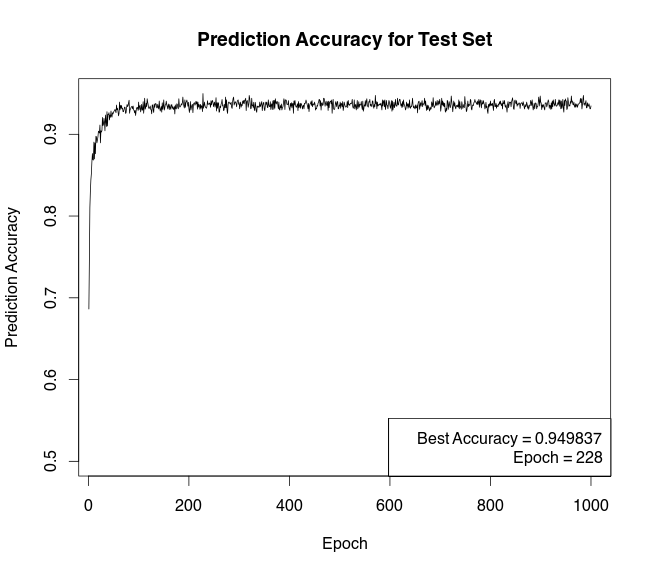
\includegraphics[width=0.6\linewidth]{Rplot.png}
\caption{ConvNet: Prediction Accuracy v.s. Number of Epochs}
\label{fig:cnn}
\end{figure}

For ConvNet we display the curve of prediction accuracy for test set w.r.t number of epochs in figure \ref{fig:cnn}, 1000 epochs in total are run for optimization. From the plot, we see that the prediction performance of Convolutional Neural Network wiggle around an certain level after 20 epochs. The best prediction accuracy is achieved at \textbf{Epoch 228} with accuracy \textbf{0.949837}, and it maintains above 0.9 after \textbf{Epoch 20}. The algorithm almost converges after 50 epochs. The total prediction accuracy after 1000 epochs is \textbf{0.9365}, The prediction accuracy for each class is much more balanced than previous methods. We can see that the Convolutional Neural Network can handle multi-class image classification well.


\section{Conclusion}
The prediction preformance of Convolutional Neural Network(accuracy = 95\%) is much better than Ensemble Method (accuracy = 85\%) for this image recognition problem, which justifies the advantage of CNN in this specific field. The good performance of Convolutional Neural Network is firstly decided by its model complexity, which is quite approriate for image recognition problem. In other words, large data set and huge feature dimension are kinds of prerequisite for the usage of Convolutional Neural Network. Moreover, the success of Convolutional Neural Network is also decided by that it captures the local structures for images, which is one of the most significant characteristics of image data. This advantage is based on the fact that convolution layer enable the local data to share the weights, which is quite different from other methods. In conclusion, Convolutional Neural Network has great advantages in image recognition problem.

\printbibliography

\section*{Appendix}
\subsection*{Implementation Details}
For Ensemble Methods, we firstly vectorzie the image and save it as .npy file. For the Convolutional Neural Network, we store the file as 4D array (d1, d2, d3, d4), where d1 stands for the number of observations, d2 stands for the number of channels, $d1 \times d2$ stands for the dimension for pixels.
We use several python modules for this project, including sklearn, Theano, xgboost and keras. The sklearn module is used for Random Forest and Restricted Bolzmann Machine pretraining. Theano is implemented for training the Deep Belief Network. The xgboost module is taken to realize the boosting algorithm. Finally, we use keras to solve the Convolution Neural Network problem with real-time data augmentation.

\subsection*{Grid Search Cross-Validation Design}
\begin{table}[ht]
\centering
\small
\caption{Grid Search CV for Gradient Boost}
\label{cv:gb}
\begin{tabular}{llll}
\toprule
number of rounds: & 100 & 500 & 1000 \\
feature proportion:     & 0.3 & 0.8 & 1   \\
maximum depth:    & 6   & 9   & 12  \\
\bottomrule
\end{tabular}
\end{table}

\begin{table}[ht]
\centering
\small
\caption{Grid Search CV for Random Forest}
\label{cv:rf}
\begin{tabular}{llll}
\toprule
number of trees: & 100 & 500 & 1000 \\
maximum feature:     &200  & 500 & 1000   \\
maximum depth:    & 6   & 9   & 12  \\
\bottomrule
\end{tabular}
\end{table}


\begin{table}[ht]
\centering
\caption{Structure of ConvNet(whole data)}
\begin{tabular}{lll}
\hline
Layer           & Size             & Output             \\ \hline
input           &                  & (32, 1, 100, 100)  \\
convolution     & 32 $3 \times 3$ kernels   & (32, 32, 100, 100) \\
convolution     & 16 $3 \times 3$ kernels   & (32, 16, 100, 100) \\
max-pooling     & $2 \times 2$, stride 2    & (32, 16, 50, 50)   \\
dropout         & p=0.25           & (32, 16, 50, 50)   \\
convolution     & 64 $3 \times 3$ kernels   & (32, 64, 50, 50)   \\
convolution     & 32 $3 \times 3$ kernels   & (32, 32, 50, 50)   \\
max-pooling     & $2 \times 2$, stride 2    & (32, 32, 25, 25)   \\
dropout         & p=0.25           & (32, 32, 25, 25)   \\
convolution     & 128 $3 \times 3$ kernels  & (32, 128, 25, 25)  \\
convolution     & 128 $3 \times 3$ kernels  & (32, 128, 25, 25)  \\
convolution     & 64 $3 \times 3$ kernels   & (32, 64, 25, 25)   \\
max-pooling     & $2 \times 2$, stride 2    & (32, 64, 12, 12)   \\
dropout         & p=0.25           & (32, 64, 12, 12)   \\
convolution     & 256 $3 \times 3$ kernels  & (32, 256, 12, 12)  \\
convolution     & 256 $3 \times 3$ kernels  & (32, 256, 12, 12)   \\
convolution     & 128 $3 \times 3$ kernels  & (32, 128, 12, 12)  \\
max-pooling     & $2 \times 2$, stride 2    & (32, 128, 6, 6)    \\
dropout         & p=0.25           & (32, 128, 6, 6)    \\
fully connected & 512 hidden units & (32, 512)          \\
dropout         & p=0.5            & (32, 512)          \\
fully connected & 256 hidden units & (32, 256)          \\
dropout         & p=0.5            & (32, 256)          \\
fully connected & 121 way soft-max & (32, 121)          \\ \hline
\end{tabular}
\end{table}


\end{document}
